\chapter*{Programme officiel}

\section*{Programme officiel}

À partir des types de base se constituent des types construits, qui sont introduits au fur et à mesure qu'ils sont nécessaires.

Il s'agit de présenter tour à tour les p-uplets (tuples), les enregistrements qui collectent des valeurs de types différents dans des champs nommés et les tableaux qui permettent un accès calculé direct aux éléments. En pratique, on utilise les appellations de Python, qui peuvent être différentes de celles d'autres langages de programmation.

{\centering\begin{tabular}{|L{3cm}|L{5.5cm}|L{6cm}|}\hline
\cellcolor{bo}\bfseries\textcolor{white}{Contenus}&
\cellcolor{bo}\bfseries\textcolor{white}{Capacités attendues}&
\cellcolor{bo}\bfseries\textcolor{white}{Commentaires}\\ \hline
p-uplets.

p-uplets nommés
&
Écrire une fonction renvoyant un p-uplet de valeurs.
& \\ \hline
Tableau indexé, tableau donné en compréhension
&
Lire et modifier les éléments d'un tableau grâce à leurs index.

Construire un tableau par compréhension.

Utiliser des tableaux de tableaux pour représenter des matrices : notation a [i] [j].

Itérer sur les éléments d'un tableau.
&
Seuls les tableaux dont les éléments sont du même type sont présentés.

Aucune connaissance des tranches (slices) n'est exigible.

L’aspect dynamique des tableaux de Python n'est pas évoqué. Python identifie listes et tableaux.

Il n'est pas fait référence aux tableaux de la bibliothèque NumPy.\\ \hline
Dictionnaires par clés et valeurs
&
Construire une entrée de dictionnaire.

Itérer sur les éléments d'un dictionnaire.
&
Il est possible de présenter les données EXIF d'une image sous la forme d'un enregistrement.

En Python, les p-uplets nommés sont implémentés par des dictionnaires.

Utiliser les méthodes keys(), values() et items().\\ \hline
\end{tabular}\par}


\chapter{Tableaux indexés}

\section{Définition et lecture}

\Cours{{\bfseries Tableau}

D'un point de vue algorithmique, un \emph{tableau} est une structure de données définie par une séquence finie d'éléments de même type, auxquels on accède par leur position (entière positive) dans la séquence, appelé indice. 
}

Le langage Python n'implémente pas directement ce type. On utilisera le type \pythoninline{list}, plus permissif (par exemple qui autorise des valeurs de types différents).

\begin{itemize}
	\item On peut définir un tableau par la séquence de ses valeurs : \pythoninline{Tableau = [15,18,20]}.
	\item Sa taille est donnée par la fonction \pythoninline{len()} : \pythoninline{len(Tableau)} vaut 3.
	\item On accède à chaque valeur par son indice (entre 0 et 2) : \pythoninline{Tableau[1]} vaut 18.
	\item Ses valeurs sont modifiables (le type tableau est mutable) : \pythoninline{Tableau[1]=12}.
	\item C'est comme si on avait trois variables : \pythoninline{Tableau[0]}, \pythoninline{Tableau[1]} et \pythoninline{Tableau[2]}.
\end{itemize}

\begin{multicols}{2}
Représentation humaine :

\begin{tabular}{|c|c|c|c|}
\hline
Tableau & 15 & 18 & 20 \\
\hline
\end{tabular}

\medskip
Implémentation (liste Python) :

\pythoninline{Tableau = [15,18,20]}.

\columnbreak
Représentation en mémoire :

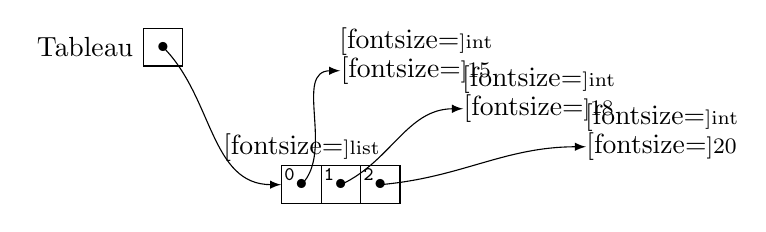
\begin{tikzpicture}
\node(T){\pythoninline{Tableau}};
\node[inner sep = 5pt, right, draw](Tc)at(T.east){\footnotesize$\bullet$};
\node[inner sep = 5pt, draw, below right = 1.5cm](L0)at(Tc){\footnotesize$\bullet$};
\draw[-latex](Tc.center)to[out = -45, in = 180](L0.west);
\node[inner sep = 1pt, below right]at(L0.north west){\scriptsize\texttt{0}};
\node[inner sep = 1pt, above]at(L0.north){\pythoninline[fontsize=\scriptsize]{list}};
\node[inner sep = 5pt, draw, right = -0.4pt](L1)at(L0.east){\footnotesize$\bullet$};
\node[inner sep = 1pt, below right]at(L1.north west){\scriptsize\texttt{1}};
\node[inner sep = 5pt, draw, right = -0.4pt](L2)at(L1.east){\footnotesize$\bullet$};
\node[inner sep = 1pt, below right]at(L2.north west){\scriptsize\texttt{2}};
\node[inner sep = 0pt,right=2.25cm, yshift=-0.3cm](V0)at(Tc){\pythoninline[fontsize=\footnotesize]{15}};
\node[inner sep = 0pt, above]at(V0.north){\pythoninline[fontsize=\scriptsize]{int}};
\node[inner sep = 0pt,below right=0.3cm, xshift=0.3cm](V1)at(V0){\pythoninline[fontsize=\footnotesize]{18}};
\node[inner sep = 0pt, above]at(V1.north){\pythoninline[fontsize=\scriptsize]{int}};
\node[inner sep = 0pt,below right=0.3cm, xshift=0.3cm](V2)at(V1){\pythoninline[fontsize=\footnotesize]{20}};
\node[inner sep = 0pt, above]at(V2.north){\pythoninline[fontsize=\scriptsize]{int}};
\draw[-latex](L0.center)to[out = 45, in = 180](V0.west);
\draw[-latex](L1.center)to[out = 25, in = 180](V1.west);
\draw[-latex](L2.center)to[out = 5, in = 180](V2.west);
\end{tikzpicture}
\end{multicols}

On peut obtenir des représentations sur : \href{http://pythontutor.com/live.html#mode=edit}{http://pythontutor.com/live.html\#mode=edit}.


\section{Itération}

Pour parcourir les valeurs d'un tableau, on peut utiliser leur indice.

\begin{multicols}{2}
Par exemple le code ci-contre affiche les valeurs du tableau en passant à la ligne après chaque bloc de quatre valeurs.

\begin{minted}{python}
valeur = [0,1,1,0,1,0,1,0,1,0,1,1]
for i in range(len(valeur)):
    print(valeur[i], end = '')
    if i % 4 == 3 : print()
\end{minted}
\end{multicols}

Mais les indices peuvent ne pas avoir d'importance et seulement surcharger l'écriture du code. Dans ce cas, on peut itérer directement sur les éléments du tableau :


\begin{multicols}{2}
Avec les indices :

\vspace{-2ex}
\begin{minted}{python}
valeur = [10,13,15,11,12]
somme = 0
for i in range(len(valeur)):
    somme = somme + valeur[i]
\end{minted}

Sans les indices :

\vspace{-2ex}
\begin{minted}{python}
valeur = [10,13,15,11,12]
somme = 0
for val in valeur:
    somme = somme + val
\end{minted}
\end{multicols}

{\bfseries Pour aller plus loin :} Il peut se produire des cas où l'on aimerait avoir les deux avantages. (Notamment si l'itération ne porte pas sur un tableau mais sur un autre itérable dont on ne sait pas déterminer facilement la taille.) On peut les obtenir avec la syntaxe suivante :


\vspace{-2ex}
\begin{minted}{python}
valeur = [10,13,15,11,12]
for (i,val) in enumerate(valeur):
    print('valeur[', i, '] = ',val, sep='')
\end{minted}

\section{Tableaux en compréhension}

On peut construire une liste Python à l'aide de la méthode \pythoninline{append()}.

\begin{multicols}{2}
Par exemple pour dresser le tableau des 10 premiers carrés d'entiers naturels, on peut écrire le code Python ci-contre.

\begin{minted}{python}
carre = []
for x in range(10):
    carre.append(x ** 2)
\end{minted}
\end{multicols}

Il existe une manière condensée de faire la même chose :\pythoninline{carre = [x**2 for x in range(10)]}

\begin{multicols}{2}
Dans l'exemple ci-contre, on utilise cette façon de faire pour appliquer un traitement à tous les éléments d'un autre tableau.

\begin{minted}{python}
lettres = ['a', 'e', 'i', 'o', 'u']
lettres = [ord(l) for l in lettres]
\end{minted}
\end{multicols}

On peut également imposer une condition à l'inclusion de la valeur : 

\pythoninline{chiffresPairs = [n for n in range(10) if n%2 == 0]}

\Cours{{\bfseries Tableau en compréhension}

On définit un tableau en compréhension en utilisant une description de ses termes.

Avec Python, elle prend la forme suivante :

\pythoninline{[fonction(item) for item in iterable if condition(item)]}

}

\section{Tableau de tableaux}

L'idée des tableaux de tableaux est de pouvoir représenter des tableaux à 2 dimensions. Par exemple, la grille d'un jeu de morpion est une grille $3\times3$. Voici deux codages possibles : \hfill\begin{tikzpicture}[scale=0.66,overlay,xshift = -3cm, yshift=-3.5cm]
\foreach \i in {0,1,2,3} \draw(0,\i)--(3,\i)(\i,0)--(\i,3);
\draw[rouge](1,1)--(2,2)(1,2)--(2,1);
\draw[bleu](1.5,2.5)circle(0.4);
\foreach \i in {1, 2, 3} \node[inner sep = 1pt, below right]at({\i-1},1){\footnotesize \texttt{\i}};
\foreach \i in {4, 5, 6} \node[inner sep = 1pt, below right]at({\i-4},2){\footnotesize \texttt{\i}};
\foreach \i in {7, 8, 9} \node[inner sep = 1pt, below right]at({\i-7},3){\footnotesize \texttt{\i}};
\end{tikzpicture}
\begin{itemize}
	\item On fait correspondre un numéro de case à un indice :
	
	     \pythoninline{[-1,0,0,0,0,1,0,0,2,0]} (1 : joueur 1 et 2 : joueur 2)

    \item On dresse la liste des cases jouées, la parité des indices donne le joueur :
    
        \pythoninline{[5,8,0,0,0,0,0,0,0]}
\end{itemize}

Voici maintenant une autre possibilité, utilisant un tableau de tableaux :\hfill\begin{tikzpicture}[scale=0.66,overlay,xshift = -3cm, yshift=-3.5cm]
\node[]at(1.5,{2.5-0}){\pythoninline{grille[0]}};
\node[]at(1.5,{2.5-1}){\pythoninline{grille[1]}};
\node[]at(1.5,{2.5-2}){\pythoninline{grille[2]}};
\foreach \i in {0,1,2,3} \draw(0,\i)--(3,\i)(\i,0)--(\i,3);
\draw[rouge](1,1)--(2,2)(1,2)--(2,1);
\draw[bleu](1.5,2.5)circle(0.4);
\end{tikzpicture}

\begin{itemize}
	\item La grille est un tableau de lignes  :
	
	\pythoninline{grille[0] = [0,2,0]}, \pythoninline{grille[1] = [0,1,0]},\pythoninline{grille[2] = [0,0,0]}
	
	C'est à dire \pythoninline{grille = [ [0,2,0], [0,1,0], [0,0,0] ]}
	
	Et on accède par exemple à la valeur 2 par : \pythoninline{grille[0][1]}.
	
\end{itemize}

Ce ne sont évidemment pas les seules options (chaque élément du tableau pourrait être une colonne, ou avec des indices dans l'autre sens, etc.)

\medskip
On peut écrire des tableaux de tableaux en compréhension :

\vspace{-2ex}
\begin{minted}{python}
grille = [[3 * ligne + colonne for colonne in range(3)] for ligne in range(3)]
\end{minted}

Et on peut itérer sur ses indices ou ses éléments par une double boucle :

\vspace{-2ex}
\begin{multicols}{2}
\begin{minted}{python}
for i in len(grille) :
    for j in len(grille[i]) :
        grille[i][j] = 0
\end{minted}

\begin{minted}{python}
for ligne in grille :
    for valeur in ligne :
        valeur = 0
\end{minted}
\end{multicols}


\chapter{p-uplets (tuples) et Dictionnaires}

Le chapitre précédent présentait les tableaux : une structure de données de taille fixe, dont les éléments sont de même type, ordonnés et accessibles par leur indice. Comme de plus ils peuvent être modifiés, on dit que c'est un type \emph{mutable}. On utilise les listes pour les représenter car elles ont des propriétés similaires avec certaines restrictions en moins. Mais d'autres types s'adaptent à d'autres situations :

\begin{center}\begin{tabular}{l|c|ccc}
type construit       & tableau & \pythoninline{list} & \pythoninline{tuple} & \pythoninline{dict} \\
\hline
valeurs de même type&\checkmark &  \textsf{X}   &   \textsf{X}   &   \textsf{X}   \\
ordonné et indicé   &\checkmark &  \checkmark   &   \checkmark   &   \textsf{X}   \\
champs nommés       &\textsf{X} &  \textsf{X}   &   \textsf{X}   &   \checkmark   \\
mutable             &\checkmark &  \checkmark   &   \textsf{X}   &   \checkmark   \\
taille fixe         &\checkmark &  \textsf{X}   &   \checkmark   &   \textsf{X}   \\
\end{tabular}\end{center}

Il existe aussi des p-uplets nommés, qui ont les mêmes caractéristiques que les p-uplets mais dont on peut nommer des champs. Dans la pratique au lycée, nous utiliserons préférentiellement les dictionnaires dans ce cas.

\section{p-uplets}

\subsection{Définition}

\Cours{{\bfseries p-uplets}

Un \emph{p-uplet} est une structure de données définie par une séquence finie d'éléments non modifiables, auxquels on accède par leur position (entière positive) dans la séquence, appelé indice.
}

 Un 2-uplet est un couple, par exemple (latitude, longitude). Un 3-uplet est un triplet, par exemple les coordonnées d'un point dans l'espace. Un 4-uplet est un quadruplet, etc.

\subsection{Fonctionnalité}

Le langage Python implémente ce type sous la dénomination \pythoninline{tuple}.

\begin{itemize}
	\item On peut définir un p-uplet par la séquence de ses valeurs : \pythoninline{point = ('A',3)}.
	\item Les parenthèses ne sont pas obligatoires, on peut aussi écrire : \pythoninline{point = 'A',3}.
	\item Pour un 1-uplet, l'absence de virgule ne permettrait pas de savoir si les parenthèses sont de simples parenthèses de calcul, ou la définition d'une structure. Python permet de terminer la séquence de valeurs par une virgule pour lever toute ambiguïté : \pythoninline{point = 'A',3,}, et pour un  1-uplet : \pythoninline{lettre = 'A',}.
	\item Pour un 0-uplet, cette notation ne suffit plus. On utilise alors : \pythoninline{vide = tuple()}.
	\item C'est, pour les mêmes raisons, la notation à utiliser pour une définition en compréhension : \pythoninline{chiffresPairs = tuple(n for n in range(10) if n%2 == 0)}
	\item Sa taille est donnée par la fonction \pythoninline{len()} : \pythoninline{len(point)} vaut 2.
	\item On accède à chaque valeur par son indice : \pythoninline{point[1]} vaut 3.
	\item Ses valeurs ne sont pas modifiables : \pythoninline{point[1]=12} provoquera une erreur.
	\item C'est comme si on avait deux constantes : \pythoninline{point[0]} et \pythoninline{point[1]}.

    \item On peut \emph{itérer} un p-uplet.


\begin{multicols}{2}
Avec les indices :

\vspace{-2ex}
\begin{minted}{python}
valeur = (10,13,15,11,12)
somme = 0
for i in range(len(valeur)):
    somme = somme + valeur[i]
\end{minted}

Sans les indices :

\vspace{-2ex}
\begin{minted}{python}
valeur = (10,13,15,11,12)
somme = 0
for val in valeur:
    somme = somme + val
\end{minted}
\end{multicols}
\end{itemize}

\subsection{Utilisation}

Le fait que ce type ne soit pas mutable peut être la propriété recherchée. 

Cela fait des données des constantes.

\medskip

Les éléments d'un p-uplet peuvent être des noms de variables (ou de fonctions). 

C'est ce qui permet les affections multiples donc les écritures comme :

\vspace{-2ex}
\begin{minted}{python}
x, y = 1, 2 # Le tuple n'est pas mutable, la variable x est toujours la variable x.
x, y = y, x # C'est la valeur que pointe (représente) x qui change !
\end{minted}

\medskip

On utilise cette structure pour permettre à une fonction de renvoyer plusieurs valeurs.

\vspace{-2ex}
\begin{minted}{python}
def divisionEuclidienne(x,y):
    return x//y, x%y
    
quotient, reste = divisionEuclidienne(7,2)
\end{minted}


\medskip
{\bfseries Pour aller plus loin : Unpacking}

On peut aussi vouloir se servir de cette structure pour passer un nombre indéterminé de valeurs à une fonction : 

\vspace{-2ex}
\begin{minted}{python}
def produit(valeurs):
    produit = 1
    for val in valeurs:
        produit = produit * val
    return produit

p = produit((1,2,3))
\end{minted}

Mais cela surcharge l'écriture de l'appel de la fonction.

On utilise alors l'opérateur \emph{splat} \pythoninline{*} pour récupérer les arguments en surnombre dans un seul un p-uplet :

\vspace{-2ex}
\begin{minted}{python}
def produit(*valeurs):
    produit = 1
    for val in valeurs:
        produit = produit * val
    return produit

p = produit(1,2,3)
\end{minted}

Dans l'appel de chacune des fonctions précédentes, la variable locale \pythoninline{valeurs} vaut la même chose : le triplet \pythoninline{(1,2,3)}.

\medskip

Cet opérateur permet de << dépacker >> un tuple. Si par exemple on dispose d'un n-uplet et qu'on souhaite l'utiliser pour les dernières valeurs d'un (n+1)-uplet :

\vspace{-2ex}
\begin{minted}{python}
coord = (3, -5)
point = ('A',*coord)  # revient à point = ('A', 3, -5)
\end{minted}

\section{Dictionnaires}

\subsection{Définition}

\Cours{{\bfseries Dictionnaire}

Un dictionnaire est une structure de données définie par un ensemble d'éléments, auxquels on accède par mot clé.}

Exemple : \pythoninline{{'nom' : 'A', 'x' : 3, 'y' :-5}} ou \pythoninline{{'nom' : 'A', 'coord' : (3, -5)}} ou encore \pythoninline{{(3, -5) : 'A'}}...

\subsection{Fonctionnalité}

Le langage Python implémente ce type sous la dénomination \pythoninline{dict}.

\begin{itemize}
	\item il est défini par l'ensemble de ses éléments (clé : valeurs) : \pythoninline{point = {'x' : 3, 'y' :-5}}. Une clé doit être unique (une clé comme un indice de liste ne référence qu'une valeur).
	\item Le dictionnaire vide s'écrit : \pythoninline{vide = dict()}.
	\item Un dictionnaire en compréhension s'écrit : \pythoninline{{n : n ** 3 for n in range(10) if n > 0}}
	\item Sa taille est donnée par la fonction \pythoninline{len()} : \pythoninline{len(point)} vaut 2.
	\item La liste des clés est \pythoninline{list(point.keys())}.
	\item La liste des valeurs est \pythoninline{list(point.values())}.
	\item La liste des couples (clé, valeur) est \pythoninline{list(point.items())}.
	\item On accède à chaque valeur par sa clé : \pythoninline{point['x']} vaut 3.
	
	Si une clé peut ne pas être présente, on utilise la méthode \pythoninline{get()} :
	
	 \pythoninline{point.get('z',0)]} renvoie \pythoninline{point['z']} si \pythoninline{'z'} est bien une clé ;  \pythoninline{0} sinon (par défaut).
	 
	 ( On peut tester la présence d'une clé avec la méthode \pythoninline{has_key()}. )
	 
	\item C'est comme si on avait plusieurs variables : \pythoninline{point['x']}, \pythoninline{point['y']}.

    \item On peut \emph{itérer} un dictionnaire par ses clés :


\begin{multicols}{2}
De manière implicite :

\vspace{-2ex}
\begin{minted}{python3}
for clef in point :
    print(clef, ':', point[clef])
\end{minted}

De manière explicite :

\vspace{-2ex}
\begin{minted}{python3}
for clef in point.key() :
    print(clef, ':', point[clef])
\end{minted}
\end{multicols}

\begin{multicols}{2}
    \item On peut itérer sur les valeurs :
    
\vspace{-2ex}
\begin{minted}{python3}
for valeur in point.values() :
    print(valeur)
\end{minted}

    \item On peut itérer sur les éléments :
    
\vspace{-2ex}
\begin{minted}{python3}
for clef, valeur in point.items() :
    print(clef, ':', valeur)
\end{minted}
    
\end{multicols}
\end{itemize}

\subsection{Exemple d'utilisation}

Cet exemple suppose que la bibliothèque \mintinline{text}{pillow} soit installée, et la présence d'une image dans le dossier de travail.

Les données EXIF d'une image sont de la forme \mintinline{text}{clé-numérique : valeur}.

Pillow contient un dictionnaire \pythoninline{TAGS} d'éléments  \mintinline{text}{clé-numérique : signification}.

\begin{minted}{python3}
from PIL import Image
from PIL.ExifTags import TAGS
 
with Image.open('image.jpg') as img:
    exif = img._getexif()
    for tag in exif :
        print(TAGS.get(tag, tag),':',exif[tag])
\end{minted}

